\title{Fun with Lines and Waves}
\date{\today}
\author{Stevo Bailey}

\documentclass[12pt]{article}

\usepackage[english]{babel}
\usepackage[utf8x]{inputenc}
\usepackage{amsmath}
\usepackage{graphicx}
\usepackage{titling}
\usepackage{caption}
\usepackage{subcaption}
%\usepackage{hyperref}
\usepackage{color}
\usepackage[normalem]{ulem}
\usepackage{titling}

\pretitle{\begin{center}\Huge\bfseries}
\posttitle{\par\end{center}\vskip 0.5em}
\preauthor{\begin{center}\Large}
\postauthor{\end{center}}
\predate{\par\large\centering}
\postdate{\par}


\usepackage{epstopdf}
\graphicspath{{./figures/}}
\DeclareGraphicsExtensions{.eps,.png,.pdf}


\newcommand{\degree}{\ensuremath{^\circ} }

\begin{document}
\maketitle

\section{Introduction}
The second lab has two distinct parts.
First the 21 cm line was measured by collecting data from the rooftop horn and averaging over time.
Since this line originates from atomic hydrogen, the most abundant molecule, it's far stronger than any other line.
A series of filters shape the spectrum and downconvert it to baseband, at which point many samples are taken over time and the noise is averaged out.
This leaves a strikingly large HI line spike.
The spectrum is further idealized by removing the filter shape and calibrating the magnitude with a blackbody (or several bodies).

Second, coaxial cables and waveguides are explored.
Coaxial cables shield signals from outside noise using a coaxial conductor.
Waveguides provide free-space signal communication.
The boundary conditions for each are different, with coax cables requiring impedance matching and waveguides requiring an open boundary.
Choosing the proper boundary prevents reflections which degrade the signal-to-noise (SNR) ratio.
Finally, the method of least squares is introduced as a way to optimally fit data to a known function.


\section{Measuring That Pesky 21 cm Line}
As mentioned earlier, the 21 cm line originates from atomic hydrogen in the Milky Way.
The abundance of atomic hydrogen means this line is strong and easy to measure.
To measure it, we used a double-heterodyne system, downconverting the 1420.4~MHz signal to 190.4~MHz and then less than 2~MHz.
Amplifiers first amplify the input signal, which is mixed to 190.4~MHz and filtered through a bandpass filter.
The mixer here has a tunable LO, allowing the signal to be placed in either sideband.
By dithering the signal's sideband placement, the filter shape can be removed from the spectrum while maintaining full SNR.
Next this signal is mixed again, downconverting it to baseband using the single-sideband technique and an LO of 190~MHz.
A simple block diagram of this system is shown in Figure~\ref{fig:bd}.

\begin{figure}
\centering
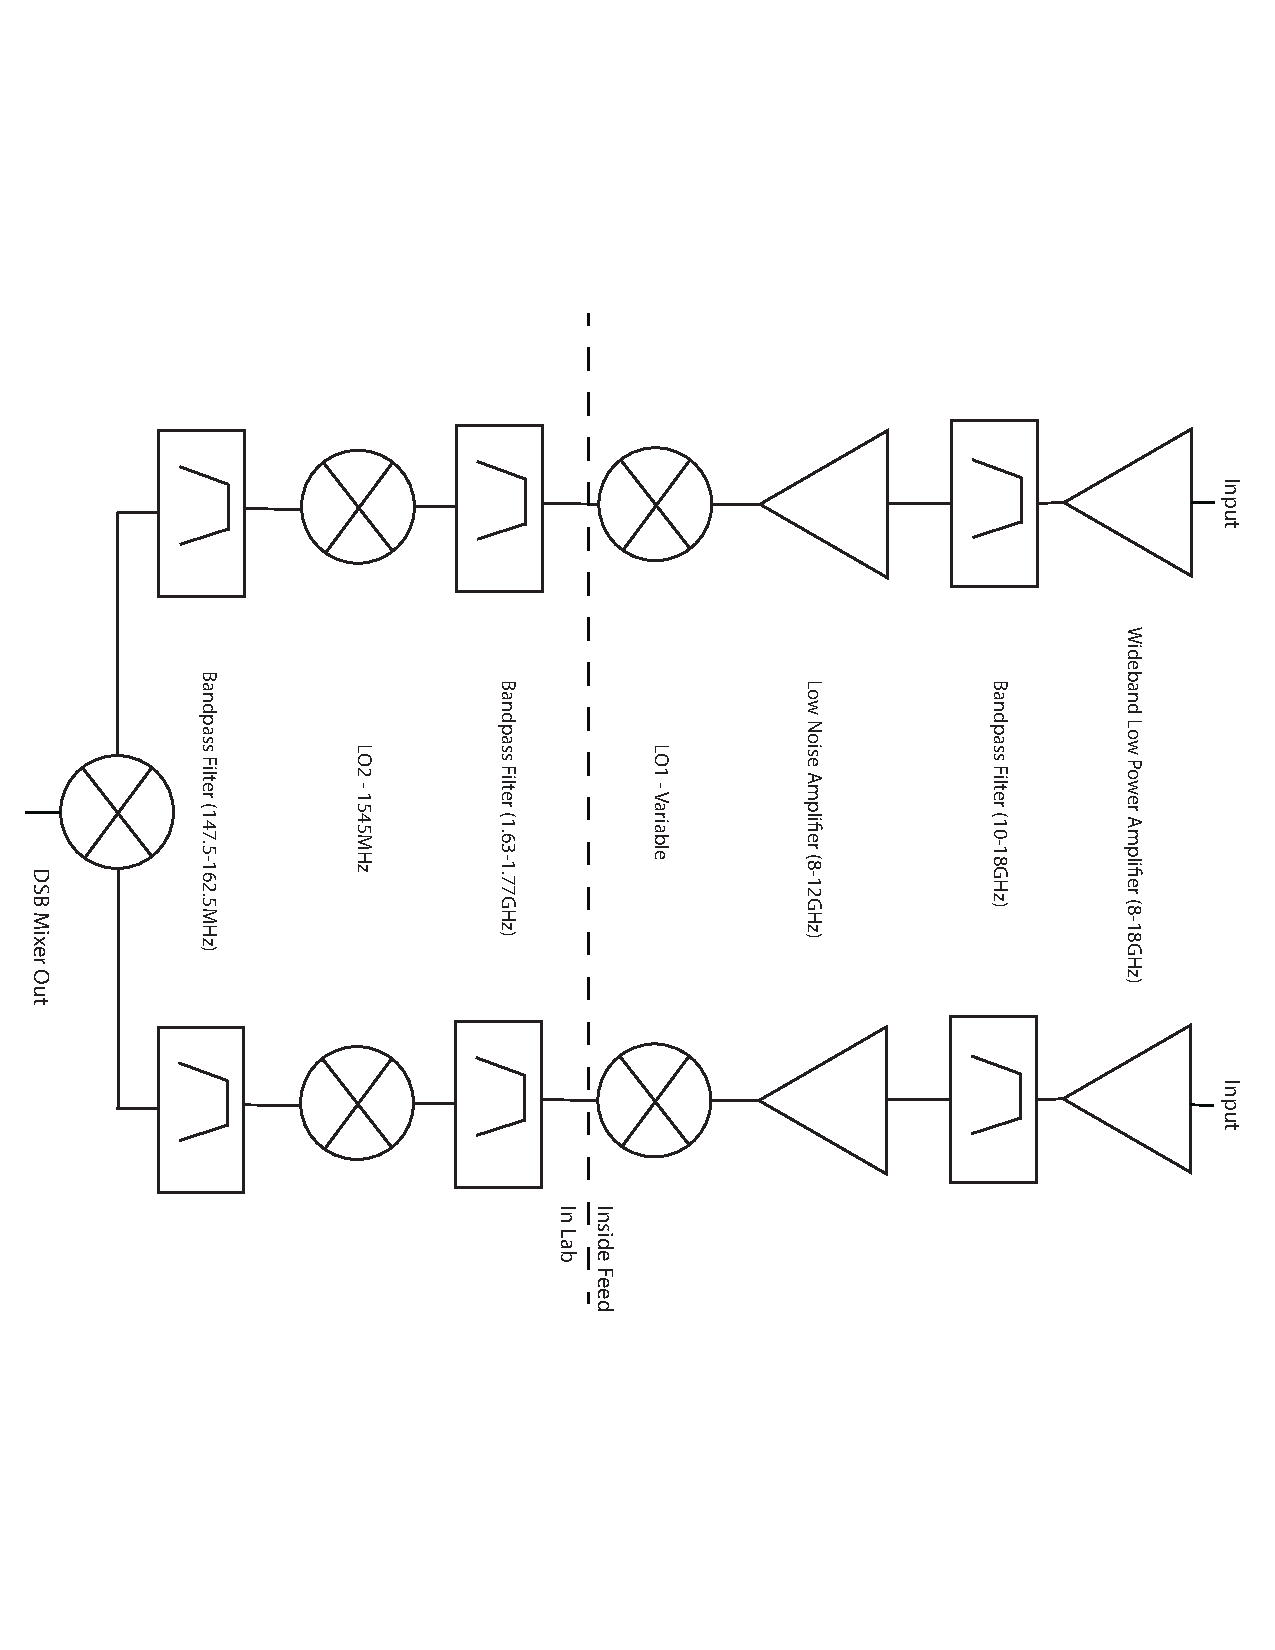
\includegraphics[width=0.95\linewidth]{bd}
\caption{Block diagram of the 21 cm line measurement system.}
\label{fig:bd}
\end{figure}

\subsection{Signal Quantization}
First, several samples were taken at different peak voltage values to determine an acceptable sampling level.
Sampling at a voltage too high will degrade signal quality and not fully utilize the available sampling range.
If the voltage is too low, the signal will saturate and get cropped.
As shown in Figure~\ref{fig:1vhist}, sampling at 1 V has lots of quantization and a range of several thousand.
Since we know the output is 16 bits, the available range is $2^{16}=65536$, so we are clearly underutilizing our range.
However, at 100 mV as in Figure~\ref{fig:100mvhist}, the range is tens of thousands but not beyond the available range, so this voltage was used for all future sampling.


% subfigure:
\begin{figure}[h]
    \centering
    \begin{subfigure}[b]{0.44\textwidth}
        \includegraphics[width=1.09\linewidth]{1v_hist}
        \caption{Max voltage of 1 V}
        \label{fig:1vhist}
    \end{subfigure}
    \quad
    \begin{subfigure}[b]{0.46\textwidth}
        \includegraphics[width=\linewidth]{100mv_hist}
        \caption{Max voltage of 100 mV}
        \label{fig:100mvhist}
    \end{subfigure}
    \caption{Voltage histograms showing quantization extent}
\end{figure}

\subsection{Data Collection and Smoothing}
To collect data, the tunable LO was set to alternate between 1229.4~MHz and 1231.4.
This placed the HI line at about 1~MHz and -1~MHz.
The two sets of data were independently averaged using either the mean or median to reduce noise, and the resultant spectra were channel-smoothed using a 10-sample median.
Figure~\ref{fig:rawspectra} shows the resultant spectra
As seen, the HI line appears in either the lower sideband (LSB) or upper sideband (USB).
Taking the average of N spectra results in less noise, since this noise is white across the sampling bandwidth.
Note large peaks, like one at DC, were removed by the 10-channel median smoothing.
However, this still leaves the filter shape.
To remove this, we can divide the two spectra.

% Figure:
\begin{figure}
\centering
\includegraphics[width=0.75\linewidth]{raw_spectra}
\caption{Spectral averages and medians with the HI line placed in either the LSB or USB.}
\label{fig:rawspectra}
\end{figure}


\subsection{Spectral Cleanup}
By taking the ratio of the two spectra (LSB and USB), the filter shape is removed.
These two spectra were shifted up to their RF frequencies and combined (averaged) to further improve the SNR.
Since taking the ratio makes the signal to appear in the other sideband, only a small frequency range is shown.
Figure~\ref{fig:rfspectrum} shows the resulting spectrum.
Now the signal has the right frequency, but the magnitude is currently arbitrary.


% Figure:
\begin{figure}
\centering
\includegraphics[width=0.75\linewidth]{rf_spectrum}
\caption{Spectrum shifted to RF, with the LSB and USB spectra combined for improved SNR.}
\label{fig:rfspectrum}
\end{figure}

To calibrate the magnitude, two spectra were taken.
One looking at the cold sky, just like our previous measurements.
For the other, several blackbodies (students) were placed in front of the horn, and a second measurement was taken.
Since students are roughly at 300K, the system temperature can now be calibrated.
Since students are roughly at 301K, the system temperature can now be calibrated.
The system temperature is given by
\begin{equation}
T_{sys}=\frac{\sum{s_{cold}}}{\sum{\left(s_{300K}-s_{cold}\right)}}T_{cal}
\end{equation}
where $T_{cal}$ = 300K and the spectra are summed over all channels.
Figure~\ref{fig:rffin} shows the final RF spectrum calibrated for the system temperature.

\begin{figure}
\centering
\includegraphics[width=0.95\linewidth]{rf_final_spectrum}
\caption{RF spectrum calibrated to the system temperature.}
\label{fig:rffin}
\end{figure}

\subsection{Doppler Effect}
Doppler correction takes into account the Doppler effect of a moving source and receiver.
Since the source is a large heap of atomic hydrogen of unknown size, source correction is impossible.
Instead, relative Doppler velocities can be found, where zero velocity occurs right at the HI line, or 1420.4~MHz.
First, the Doppler velocity was found by using the standard Doppler formula, 
\begin{equation}
\frac{v}{c}=-\frac{\Delta f}{f_0}.
\end{equation}
Figure~\ref{fig:rfdop} shows the calibrated spectrum plotted against the Doppler velocity.
Lastly, the velocity was corrected for the motion of the Sun and also adjusted to the Local Standard of Rest (LSR) frame.
On the day of observation, the barycentric reference frame was moving at 18.77~km/s away from the zenith, and the LSR was moving away at 20.37~km/s away.
Figures~\ref{fig:rfbary} and ~\ref{fig:rflsr} show the adjusted velocities for these two reference frames.
Because the velocities are so similar, the plots look nearly identical.

\begin{figure}
\centering
\includegraphics[width=0.95\linewidth]{rf_dop_spectrum}
\caption{Calibrated power spectrum plotted against the Doppler velocity.}
\label{fig:rfdop}
\end{figure}

\begin{figure}
\centering
\includegraphics[width=0.75\linewidth]{rf_bary_spectrum}
\caption{Calibrated power spectrum plotted against the velocity of the barycentric reference frame.}
\label{fig:rfbary}
\end{figure}

\begin{figure}
\centering
\includegraphics[width=0.75\linewidth]{rf_lsr}
\caption{Calibrated power spectrum plotted against the velocity of the LSR reference frame..}
\label{fig:rflsr}
\end{figure}

\section{Communication Methods}
Transmitting data accurately, efficiently, and precisely is difficult.
Measuring nonidealities in wires is important for characterizing a wire's performance and calibrating data for transmission issues.
In particular, reflections in a wire introduce systemic noise that masquerade as rogue signals or aliases.
This section of the lab explores coaxial cables and waveguides.

\section{The Coaxial Cable}
A coaxial cable shields a signal from outside noise by surrounding the signal with another conductor acting as a Faraday cage.
This experiment used a slotted line and a 3~GHz signal to explore how standing waves behave in a coaxial cable.
The peaks and troughs of a signal passing through the cable were noted when one end was open and separately when one end was closed.
With one end of the cable open, clear waves appear.
With that end closed (shorted), the signal is nearly gone.
This is because the shorted end prevents reflections through impedance matching, so standing waves are not established. 

For the open condition, the differences between nulls were calculated.
First, the differences were naively averaged, giving an approximate wavelength of 0.1003~m.
However, since we know the null positions should increase linearly with distance, we can use least squares to fit the data to the following equation:
\begin{equation}
x_m=A+m\frac{\lambda}{2}.
\end{equation}
Doing so gives a wavelength of 0.100082~m.
The velocities are then $3.009\times 10^8$~m/s and $3.002\times 10^8$~m/s.
The least squares approaches produces an answer closer to the speed of light, which is presumably the correct answer.

The VSWR of the coaxial cable was one with a matched load. 
The load resistance was 49.8 $\Omega$.
The point of load matching is to remove reflections, which means the maximum and minimum voltages are the same.


\subsection{The Waveguide}
The waveguide had the opposite VSWR.
Its VSWR was one when one end was left open and zero when one end was closed.
For a waveguide, the ``wire" already matches the impedance of the air on one end, since the wire is air.
Thus closing one end with a conductor introduced an impedance mismatch, which explodes the VSWR to infinity.

Next, wave measurements were made with the waveguide.
Data were borrowed from team CRAM, since the frequency synthesizer was gone when we tried to take measurements.
Data were taken from 7.5~GHz to 8.75~GHz, so all data were above the expected cutoff frequency of 7~GHz.
With the waveguide end shorted, Figure~\ref{fig:wgvel} shows the signal velocities inside the waveguide.
Note the velocities are much larger than the speed of light, but this is acceptable since they represent phase velocities.
No information is transferred faster than light.
Wavelength measurements are in shown in Figure~\ref{fig:wgwl}, along with the least-squares fit.
This fit was extended down to 7~GHz, the cutoff frequency.
At 7~GHz, the wavelength is approximately 9~cm, so the waveguide has a cutoff wavelength (width) of about 9~cm.

\begin{figure}
\centering
\includegraphics[width=0.8\linewidth]{wgvel}
\caption{Phase velocities of signals within the waveguide with one end closed.}
\label{fig:wgvel}
\end{figure}

\begin{figure}
\centering
\includegraphics[width=0.8\linewidth]{wgwl}
\caption{Wavelengths of signals within the waveguide, and the least-squares fit.}
\label{fig:wgwl}
\end{figure}

\section{Conclusion}
This lab combined the knowledge of the first lab into a real system.
The system was used to measure the HI line in our galaxy.
Astronomical spherical coordinate systems and date-time systems were introduced.
The HI line was extracted by accounting for nonidealities in the filter shapes, noise in the signal, and relative velocities of the Earth and Sun.
Additionally, coaxial cables and waveguides were explored.
These communication means impose restrictions on a system, requiring impedance matching to eliminate reflections.


\enddocument
